\section{Alimentation}
Nous avons vu que la remorque utilise une prise 13 broches pour son alimentation. Le véhicule tractant la remorque peut varier, il n'y a donc pas de
garanti qu'il y ait une deuxième prise disponibles pour le système qui sera ajouté. L'idéal serait d'avoir accès au 12[V] et à la masse.
\begin{figure}[H]
    \centering
    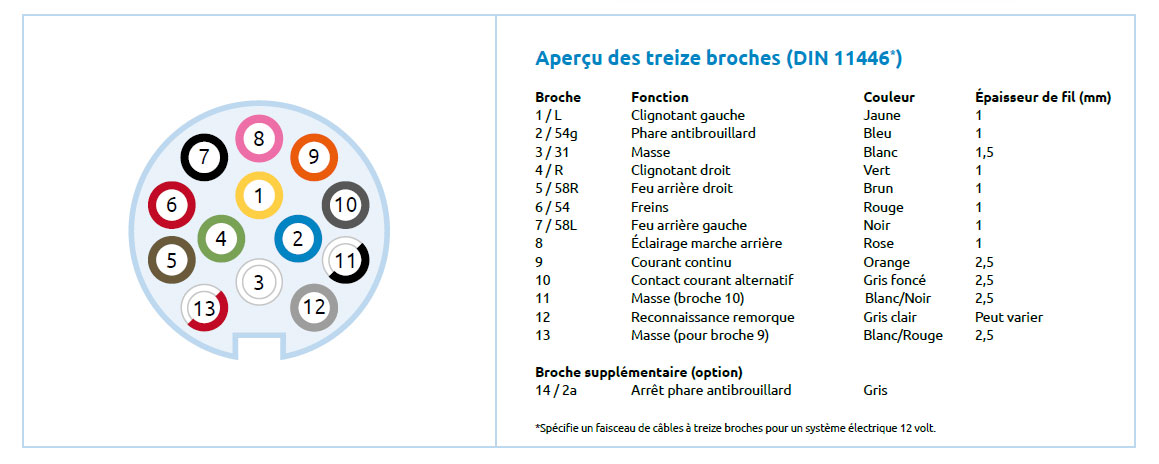
\includegraphics[width=14cm]{assets/figures/broches.jpg}
    \caption{Sortie prises 13 broches - \cite{prise}}
\end{figure}
Ce qui nous intéresse:
\begin{itemize}
    \item Broche 9  : 12 [V]
    \item Broche 13 : Masse
\end{itemize}
Les broches ayant chacune une fonction particulière, il n'existe pas de multiprise permettant de joindre deux connecteurs mâle vers une femelle.
Il faudrait donc fabriquer un boitier d'adaptation ou bricoler une rallonge permettant de dévier les broches utiles, tout en préservant l'alimentation de la remorque et du matériel installé dessus.


Voir figure \ref{alim}.
\begin{figure}[h]
    \centering
    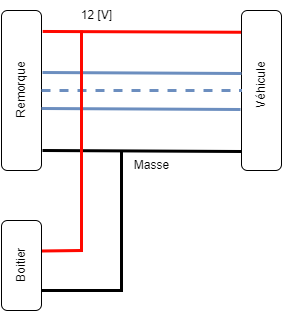
\includegraphics[height=7cm]{assets/figures/alimentation.png}
    \caption{Boitier d'adaptation de l'alimentation \label{alim}}
\end{figure}
\newpage

\section{Communication}
Dans le cadre de ce projet, plusieurs éléments devront communiquer entre eux, notamment l'unité de traitement d'image,
l'actionnement de la télécommande ainsi que le retour vidéo pour le copilote, il est donc important de définir comment ils communiqueront entre eux.
Il est important de se rappeler que leurs emplacements seront les suivants:

\begin{table}[h]
    \begin{center}
        \caption{Liste des éléments et emplacements}
        \begin{tabular}{|c|l|}
            Eléments                        & Emplacement            \\ \hline
            Caméra et boitier de traitement & Support de la remorque \\
            Eclairage                       & Timon                  \\
            Actionnement de la télécommande & Support de la remorque \\
            Affichage pour copilote         & Dans le véhicule
        \end{tabular}
    \end{center}
\end{table}

Dans notre cas de figure, les éléments sont concentrés sur la remorque et dans le véhicule tractant. La communication câblée est possible
entre la caméra, le boitier, l'actionnement de la télécommande et éventuellement l'éclairage si celui-ci à besoin d'être contrôlé spécifiquement.
En ce qui concerne le retour vidéo, il se trouvera principalement dans l'habitacle du véhicule, mais pourrait également être emporté autour du véhicule,
dans ce cas, la connexion filaire n'est pas envisageable.

Parmi les connexions sans fil:
\begin{itemize}
    \item Via une connexion Bluetooth.
    \item Via un réseau \Gls{wifi} local.
\end{itemize}
La connexion sans fil doit garantir une connectivité stable sur un rayon de 5 mètres autour du véhicule (avec obstacles). De plus, le débit doit être
suffisant pour diffuser un flux vidéo. La solution du réseau local \Gls{wifi} semble être la meilleure.

\textbf{La possibilité de communiquer via un réseau local \Gls{wifi} devient donc un prérequis pour le retour vidéo.}
\newpage
\section{Capture et traitement d'image}
\subsection{Eclairage}
La sélection de l'éclairage va dépendre des points suivants:
\begin{itemize}
    \item La longueur d'onde nécessaire.
    \item L'emplacement de l'éclairage
    \item La taille du champ à éclairer.
\end{itemize}
Le premier point s'est défini durant la phase de recherche, l'idéal serait d'avoir une source émettant une onde de 850 \si{\nano\metre}.

Les deux points suivants sont liés, l'éclairage sera monté sur le timon et le but est d'éclairer le sol sur une largeur d'environ 150 \si{\centi\metre} (correspondant aux champ d'actions du semoir),
c'est à dire sur une bande. Avec des leds montées en ligne, il n'est pas nécessaire qu'elles aient un grand angle de diffusion.

Des leds trouvées sur le site de Mouser semblent correspondre à ces conditions \cite{ledIR}.

Leur préparation se résumerait à une mise en bande sur une structure solide (2x 75\si{\centi\metre}) et les alimenter.


\subsection{Caméra}
La caméra à choisir doit remplir les critères suivants:
\begin{itemize}
    \item Pas de filtre IR (ou facilement retirable).
    \item Compatible avec une carte de traitement d'image.
    \item Champ de vision suffisant pour observer la largeur de la route.
\end{itemize}

La caméra Module 3 "NoIR - Wide" de Raspberry Pi \cite{camera} répond aux critères. Avec une mise au point à partir de 5cm vers l'infini,
une résolution de 11.9 mégapixels (4608x2592) et d'un champ de vision de \ang{120}, elle offre une image nette et très détaillée avec beaucoup de liberté sur
son placement. Sa sensibilité aux infrarouges monte jusqu'au environ de 1000 \si{\nano\metre}. Elle est disponible très rapidement et pour 30 \gls{chf}.
\begin{figure}[H]
    \centering
    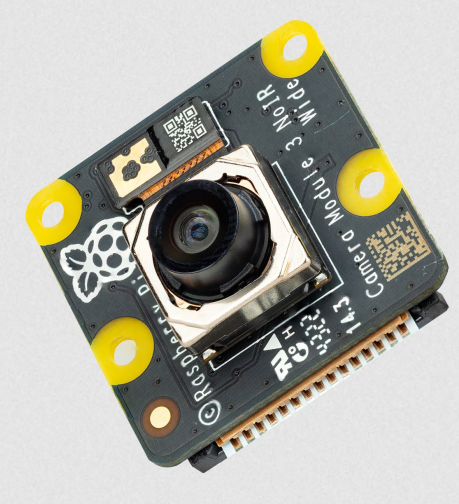
\includegraphics[height=7cm,angle=-90]{assets/figures/camera.png}
    \caption{Camera module 3 NoIR wide}
\end{figure}
\newpage
\subsection{Système embarqué de traitement}
L'unité de traitement doit respecter les contraintes suivantes:
\begin{itemize}
    \item Peu encombrant.
    \item Suffisamment puissant pour traiter les images et agir.
    \item Communication WiFi en tant qu'émetteur.
    \item Compatible avec la caméra.
\end{itemize}
En faisant une recherche rapide, on se rend compte qu'il y a beaucoup d'options parmi les marques de nano ordinateur,
et chacune des marques ont une multitude de sous-modèle.
\begin{itemize}
    \item Raspberry Pi.
    \item Intel.
    \item NanoPC.
    \item LattePanda.
    \item NVIDIA.
    \item Et beaucoup d'autres...
\end{itemize}
De manière général, la commande de nano ordinateur est très compliquée actuellement (mars 2023), il faut compter plusieurs semaines voir plusieurs mois
pour espérer recevoir quelque chose. Il est important de noter que j'effectue mon travail de Bachelor à temps plein, en 11 semaines consécutives.
Je ne peux donc pas me permettre d'attendre autant de temps pour recevoir un élément.

En m'informant sur le matériel disponible dans l'école, j'ai appris que le \Gls{reds} prêtait des Raspberry Pi 4.
J'ai donc basé ma sélection sur la disponibilité de l'élément et non pas sur ses capacités.

\textbf{Un Raspberry Pi4 4Go sera utilisé pour la suite du projet.}

Note: Le Raspberry Pi 4 sera abrévié "\Gls{rpi4}" dans la suite du rapport.

\begin{figure}[H]
    \centering
    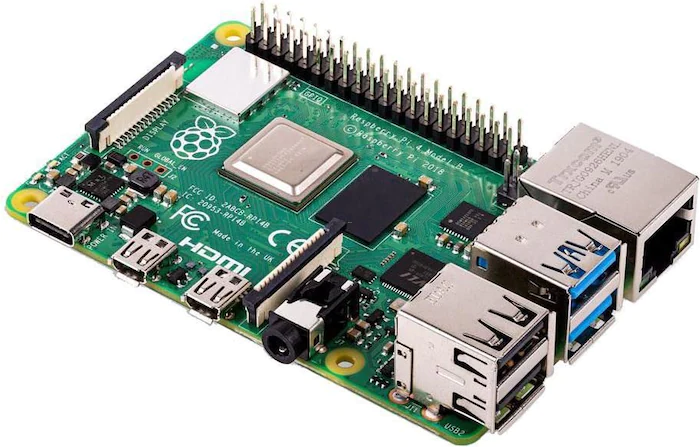
\includegraphics[height=7cm]{assets/figures/rpi4.png}
    \caption{Raspberry Pi4 4Go}
\end{figure}

\newpage
\section{Système de commande - Actionnement de la télécommande}
Les idées de base d'actionneurs permettant d'appuyer sur la télécommande sont les suivants:
\begin{itemize}
    \item Vérins électriques.
    \item Servomoteurs.
    \item Moteurs pas à pas.
    \item Aimants de levage.
\end{itemize}

Les vérins électriques ont l'avantage d'être facile à installer, il suffirait d'une plaque de support perforée au dessus de chaque bouton et d'y insérer
les pièces à la profondeur souhaitée, puis de les actionner/rétracter pour appuyer ou non sur un bouton. Cependant, les vérins disponibles sur le marché semblent être surdimensionnés pour la tâche en question, les forces et
consommation pour un fonctionnement normal sont très grand. Les prix sont également très élevé, il est difficile de trouver des pièces de moins de 100 \Gls{chf} l'unité
pour les dimensions désirées. De plus, les délais de livraison durant la période dédiée au développement de se projet sont relativement incertains pour se genre de pièce.

L'idée, avec les servomoteurs, serait de les équiper d'un élément de préhension tangent à l'axe de rotation du moteur permettant de presser sur les boutons.
Le pilotage d'un servomoteur se fait par PWM, nécessitant donc qu'une seule sortie par éléments au niveau de la carte de commande. De plus, il est assez facile de
trouver des servomoteurs avec des caractéristiques en phase avec le projet, c'est à dire d'un point de vu taille, force et consommation, et ce à des prix
raisonnables (avoisinant 10 \Gls{chf}). L'installation sur un support est plus complexe que pour les vérins.

L'utilisation du moteur pas à pas serait similaires au servomoteur, c'est à dire avec un élément qui presse sur les boutons.
Il est assez facile de trouver des moteurs avec des caractéristiques en phase avec le projet à des prix raisonnable (avoisinant 10 \Gls{chf}). La commande d'un moteur pas à pas
se fait usuellement via un pilote servant d'interface entre le moteur et la carte de commande. Il est nécessaire d'avoir une carte pilote par moteur (environ 10 \Gls{chf} par unité).
L'installation sur un support est plus complexe que pour les vérins.

Les aimants de levage, tout comme les vérins ont l'avantage d'être très simple à installer/disposer. Le prix varie suivant la taille, la pression et l'alimentation de l'aimant.
Selon la force nécessaire à l'activation du bouton, le modèle qu'il faudrait utiliser coûte environ 20 \Gls{chf}. L'activation de l'aimant peut se faire via un relai dont le contrôle
pourrait se faire via les pins I/O du \Gls{rpi4}.

Avec ces informations, en comparant prix, facilité d'acquisition, pilotage, caractéristiques obtenables, délai de livraison et facilité d'installation, la solution de l'aimant de levage semble être la plus
appropriée. J'ai trouvé un aimant de levage avec les caractéristiques suivantes:
\begin{itemize}
    \item Tension de fonctionnement: 12 \si{\volt}
    \item Puissance nominale: 7 \si{\watt}
    \item Longueur de déploiement: 10 \si{\milli\metre}
    \item Force en fin de course: 11 \si {\newton}
\end{itemize}

Un test de préhension est effectué au chapitre \ref{aimant}, le test montre que la caractéristique de force de l'aimant n'est pas suffisante.

\section{Retour vidéo}
Le résultat de l'analyse du traitement d'image et la mise en évidence des traces d'hydrocarbures doivent être visible par le conducteur/copilote.
La visualisation du retour se fera naturellement via un écran. Les idées de bases sont les suivantes:
\begin{itemize}
    \item Installation d'un écran portable.
    \item Affichage via une application mobile.
    \item Affichage via une page web locale.
\end{itemize}

Les problèmes de l'écran portable sont multiples, notamment l'alimentation, le câblage vers une source d'alimentation peut-être encombrant
et limiterait les mouvements/déplacements de l'utilisateur. De plus la connexion vers un réseau \Gls{wifi} local n'est pas garantie.

L'idée de l'application mobile présente certains avantages, comme l'installation unique. L'opérateur n'aurait qu'à mettre l'application
qu'une seul fois sur son téléphone portable pour accéder au retour vidéo (sous condition d'être connecté au réseau \Gls{wifi} local).
Tout le monde serait alors équiper de son propre écran, petit, pratique et peu encombrant. Le problème majeur est la différence de système d'exploitation
entre les téléphones portables. Le développement d'une application universelle est compliquée, il faudrait avoir une application par système grand public.
De plus, l'installation d'une application non reconnu nécessite des autorisations spéciales sur le téléphone de l'utilisateur.

L'affichage du retour vidéo via une page locale semble être optimal. En plus de regrouper les avantages de l'application mobile, nous nous débarrassons des défauts.
L'accès au lien de la page pourrait se faire via un QR code à scanner sur le boitier de commande.

\textbf{L'affichage se fera via une page web locale.}

\section{Résumé des décisions}
\begin{table}[H]
    \begin{center}
        \caption{Table de résumé des décisions}
        \begin{tabular}{|c|l|}
            Eléments                  & Solutions                         \\ \hline
            Communication             & Filaire + Réseau \Gls{wifi} Local \\
            Eclairage                 & Leds IR 850 \si{\nano\metre}      \\
            Caméra                    & Rpi module 3 NoIR Wide            \\
            Traitement d'image        & Raspberry Pi 4                    \\
            Actionnement télécommande & \textbf{A définir}                \\
            Affichage pour copilote   & Page web local                    \\
        \end{tabular}
    \end{center}
\end{table}
\newpage
\section{Bilan de consommation}
Dans le but d'installer le système sur la remorque, il est important d'avoir une idée de la consommation totale du système afin de dimensionner
un fusible à l'entrée du boitier.

\begin{table}[H]
    \begin{center}
        \caption{Table - Bilan de consommation}
        \begin{tabular}{|c|c|c|c|}
            Eléments                  & Conso. par unité   & Quantité & Conso. totale        \\ \hline
            Camera + \Gls{rpi4}       & 15 \si{\watt}      & 1        & 15    \si{\watt}     \\
            Leds IR                   & 3 \si{\milli\watt} & 100      & 300 \si{\milli\watt} \\
            Actionnement télécommande & -                  & 6*       & -                    \\
            Total                     & -                  & -        & 15.3 \si{\watt}      \\
        \end{tabular}
    \end{center}

    *Normalement, seul actionneurs peuvent être actifs simultanément.
\end{table}

Sachant que l'alimentation depuis la remorque est de 12 \si{\volt}, on en déduit que le courant sera de \(I = P/U = 15.3/12 = 1.275 \si{\ampere} \).
L'utilisation d'un fusible de 1.5 \si{\ampere} semble être une bonne option, cette valeur est disponible au \gls{fablab}. Par la suite, il serait judicieux
d'installer un disjoncteur réarmable afin d'éviter de changer de pièce en cas de problème.

\textbf{À noter que la valeur du courant nécessaire ne tient pas compte des actionneurs de la télécommande. Ce courant devra être recalculé lorsque
    cette aspect sera défini.}